\documentclass[a4,center,fleqn]{NAR}
\copyrightyear{2015} 
\pubyear{2015}
\usepackage{booktabs}
\usepackage{colortbl, xcolor}
\usepackage{tabularx}
\usepackage{multirow}
\pubdate{31 July 2009}
\pubyear{2009}
\jvolume{37}
\jissue{12}

\bibpunct{(}{)}{,}{n}{,}{,}

\newcommand*{\bigcdot}{\raisebox{-0.25ex}{\scalebox{1.5}{$\cdot$}}}

\begin{document}

\title{Prediction of amyloidogenicity based on the n-gram analysis}

\author{Micha\l{} Burdukiewicz\,$^{1}$, Piotr Sobczyk\,$^{2}$, 
Stefan R\"{o}diger\,$^{3}$,
Anna Duda-Madej\,$^{4}$,
Pawe\l{} Mackiewicz\,$^{1}$ and Ma\l{}gorzata Kotulska\,$^{5}$
\footnote{To whom correspondence should be addressed.
Email: malgorzata.kotulska@pwr.edu.pl}}

\address{
$^{1}$University of Wroc\l{}aw, Department of Genomics,
$^{2}$Wroc\l{}aw University of Science and Technology, Department of Mathematics 
$^{3}$Brandenburg University of Technology Cottbus-Senftenberg, Institute of Biotechnology
$^{4}$Wroclaw Medical University, Department of Microbiology
and 
$^{5}$Wroc\l{}aw University of Science and Technology, Department of Biomedical 
Engineering, Faculty of Fundamental Problems of Technology
}

\history{Received on XXXXX; revised on XXXXX; accepted on XXXXX}

\maketitle

\begin{abstract}
Text. Text. Text. Text. Text. Text. Text. Text. Text. Text. Text.
Text. Text. Text. Text. Text. Text. Text. Text. Text. Text. Text.
Text. Text. Text. Text. Text. Text. Text. Text. Text. Text. Text.
Text. Text. Text. Text. Text. Text. Text. Text. Text. Text. Text.
Text. Text. Text. Text. Text. Text. Text. Text. Text. Text. Text.

\end{abstract}

\section{Introduction}


Amyloid aggregates have been observed in tissues of people suffering from various diseases, such as: Alzheimer's, Parkinson's, amyotrophic lateral sclerosis and Huntington's, as well as many other conditions. These aggregates were also detected in diseases other than neurological, for example in diabetes of type 2 or certain types 
of a cataract. Cells in tissues with amyloid fibrils exhibit very high 
mortality. However, the mechanisms of the cytotoxicity have not been 
discovered. 
The aggregates are very stable and their dissolution is very difficult. Amyloids are 
resistant to activity of proteolytic enzymes and chemical compounds due to the 
specific and highly ordered structure of their steric zipper. However, some strategies to prevent amyloid formation have been proposed~\citep{hard_inhibition_2012}.

  The aggregation occurs when a cell environment fosters the partial unfolding 
of protein chains or their fragmentation in such a way that the parts prone to 
joining with other protein fragments become exposed. For the majority of proteins, 
considerable conformational rearrangement must have occurred to initiate the 
aggregation process. Such changes cannot take place in the typical tightly 
packed native protein conformation due to the constraints of the tertiary 
structure. Thus, the formation of a non-native partially unfolded conformation is 
required to start the aggregation presumably by enabling specific intermolecular interactions including electrostatic attraction, hydrogen bonding and hydrophobic contacts. This partial unfolding can be influenced by various factors, such as high 
concentration of proteins, high temperature, low pH, binding metals, or exposition to UV 
light.

  Initially, the resulting molecules form clusters consisting of a few 
elements, which are called oligomers. Next, they grow into larger aggregates. 
The aggregation of proteins or their fragments may lead to amorphous (unstructured) 
clusters or amyloid (highly ordered) unbranched fibrils. Independently of the 
protein sequence and its original structure, aggregates always display a common 
cross-$\beta$ structure. The distinctive structure of the steric zipper enables 
the selective detection of amyloids from amorphous aggregates using either a 
variety of microscopic techniques or fluorescence of probes with which they 
form compounds.

    Currently, it is believed that short peptide sequences of amyloidogenic 
properties, called hot spots, are responsible for the aggregation of amyloid 
proteins. Previous studies have suggested that amyloidogenic fragments may 
have regular characteristics, not only with regard to averaged physicochemical 
properties of their amino acids, but also the order of amino acids in the 
sequence. 
% * <pamac@smorfland.uni.wroc.pl> 2016-05-24T11:47:48.739Z:
%
% > sequence
%
% Here citation
%
% ^ <pamac@smorfland.uni.wroc.pl> 2016-05-24T11:48:12.626Z.
It is important to distinguish between amyloidogenic and amyloidic 
regions because only the former initiate the process of the aggregation and the latter consist of all regions involved in the creation of the final aggregate. Several computational approaches were proposed to model and predict both kinds of regions. Physics- and chemistry-based models used in  FoldAmyloid~\citep{garbuzynskiy_foldamyloid:_2010} utilize the density of the protein contact sites. Other methods perform threading a peptide on an amyloid fiber backbone, followed by determination of 
its energy and stability~\citep{goldschmidt_identifying_2010, 
bryan_stitcher:_2012, odonnell_method_2011}. Statistical approaches include 
production of frequency profiles, such as the WALTZ method 
\citep{beerten_waltz-db:_2015} and machine learning methods, which have been 
developed by our team \citep{stanislawski_machine_2013, gasior_fish_2014}. 
AGGRESCAN3D has been proposed to estimate more accurately aggregation 
propensity by performing 3D structure based analysis~\citep{zambrano_aggrescan3d_2015}. 

\enlargethispage{-65.1pt}

  The majority of methods described above uses theoretical knowledge to 
specify decision rules determining the presence of the hot spot. The aim of our 
study is opposite, because out of thousands of created hot spot models, we choose 
the most appropriate.
  
  In bioinformatics, n-grams (k-mers) are continuous or discontinuous sequences of 
$n$ elements. Employed as a feature extraction method, n-grams are widely used 
in analysis of biological sequences. Our choice of n-grams was driven by their 
highly interpretable nature. This is a valuable feature because we are 
interested in identification of motifs that are most relevant to amyloidogenic 
properties of peptides. The most discriminating n-grams were extracted using a 
novel feature selection algorithm called Quick Permutation Test (QuiPT).

  Several studies highlighted that three-dimensional protein structure depends 
not on the exact sequence of amino acids but on their general physicochemical 
properties. Hence, a reduction of 20 amino acid alphabet by an appropriate encoding 
amino acids into more general symbols can still retain the information about the 
protein folding~\citep{murphy_simplified_2000}. Since amyloid aggregates, 
especially their hot spots regions, have very specific spatial organization, we 
investigated if these regions can be also described by a shorter amino acid alphabet
(encoding). Instead of relying on the general similarities of amino acids, we created 
multiple encodings based on the combinations of various physicochemical properties that 
might be associated with amyloidogenicity.  

  To discover amino acid patterns specific for amyloidogenic peptides we based our 
analysis on n-grams, continuous or discontinuous sequences of length $n$. Extraction of 
n-grams allows detection of more elaborated motifs, but creates very large features spaces. 
Henceforth, we used Quick Permutation Test (QuiPT) to select only informative n-grams 
drawn from peptides encoded with the reduced amino acid alphabet.

  We used selected n-grams to train a predictor based on random forest~\citep{breiman_random_2001}
discriminating between amyloidogenic and non-amyloidogenic peptides. We trained several iterations of a 
classifier using peptides with different length to identify the optimal number of 
residues which include the information about the presence or absence of hot spots. 
In the cross-validation setup we found the encoding associated with the best-performing 
classifier and its set of informative n-grams.

\section{Methods}
\subsection{Data set}

The data used in the study was extracted from AmyLoad data 
base~\citep{wozniak_amyload:_2015}. We obtained 418 
amyloidogenic peptides and 1039 non-amyloidogenic peptides.

  Sequences shorter than six and longer than 25 amino acid residues 
(i.e., 8 and 27 sequences, respectively) were 
removed from the set. The former were too short to be processed in the
devised n-gram analysis framework and the latter were too diversified and rare, 
hampering the proper analysis.

  The final data set contained in total 1430 peptides: 397 amyloidogenic 
and 1033 non-amyloidogenic sequences. 

\subsection{Encodings of amino acids}

The amyloidogenicity of a given peptide may not depend on the exact sequence of 
amino acids but on its more general properties. To verify this hypothesis, we 
handpicked 20 measures from AAIndex database~\citep{kawashima_aaindex:_2008} 
describing features important in the  amyloidogenicity, such as: size of residues, 
hydrophobicity, solvent surface area, frequency in $\beta$-sheets and contactivity. 
We selected them among properties that were introduced after 
1980 when, thanks to the technological advancements, the measurements were more 
accurate than the older ones. The set of selected physicochemical properties was
enriched by six measures representing amino acid contact site 
propensities~\cite{wozniak_characteristics_2014} giving in total 26 features.

  Since highly correlated measures would create very similar amino acid encodings, we further 
reduced the number of properties to 17 by selecting measures with the absolute value of 
Pearson's correlation coefficient smaller than 0.95 (Tab.~\ref{tab:properties}). 

  Based on that, we created 524,284 amino acid encodings 
with different level of amino acid alphabet reduction from three to six amino acid groups 
using Ward's clusterization ~\citep{joe_h._ward_jr_hierarchical_1963},  which was performed 
on all combinations of the normalized values of physicochemical properties from 1 to 17. 

  The majority of encodings had at least one duplicate. In such case, only a 
single representative was included in the cross-validation. After filtering the 
duplicates, we obtained 18,535 unique encodings.

\begin{table}[bth]
\caption{Selected 17 physicochemical properties used to create amino acid encodings.} 
\label{tab:properties}
\small
\begin{tabularx}{\columnwidth}{@{} lX @{}}
  \toprule
  Category & Property \\ 
  \midrule
  Contactivity & Average flexibility indices \citep{bhaskaran_positional_1988} 
\\ 
  \rowcolor[gray]{0.85}Contactivity & 14 {\AA} contact number 
\citep{nishikawa_radial_1986} \\ 
  Contactivity & Accessible surface area \citep{radzicka_comparing_1988} \\ 
  \rowcolor[gray]{0.85}Contactivity & Buriability \citep{zhou_quantifying_2004} 
\\ 
  Contactivity & Values of Wc in proteins from class $\beta$, \newline  cutoff 
12 A, separation 5 \citep{wozniak_characteristics_2014} \\ 
  \rowcolor[gray]{0.85}Contactivity & Values of Wc in proteins from class 
$\beta$, \newline  cutoff 12 A, separation 15 
\citep{wozniak_characteristics_2014} \\ 
\hline 
  $\beta$-frequency & Average relative probability of inner \newline beta-sheet 
\citep{kanehisa_local_1980} \\ 
  \rowcolor[gray]{0.85}$\beta$-frequency & Relative frequency in $\beta$-sheet 
\citep{prabhakaran_distribution_1990} \\ 
  $\beta$-frequency & Thermodynamic $\beta$-sheet propensity 
\citep{kim_thermodynamic_1993} \\ 
\hline 
 \rowcolor[gray]{0.85} Hydrophobicity & Hydrophobicity index 
\citep{argos_structural_1982} \\ 
  Hydrophobicity & Optimal matching hydrophobicity 
\citep{sweet_correlation_1983} \\ 
  \rowcolor[gray]{0.85}Hydrophobicity & Hydrophobicity-related index 
\citep{kidera_statistical_1985} \\ 
  Hydrophobicity & Scaled side chain hydrophobicity values 
\citep{black_development_1991} \\ 
\hline 
  \rowcolor[gray]{0.85}Polarity & Polarizability parameter 
\citep{charton_structural_1982} \\
  Polarity & Mean polarity \citep{radzicka_comparing_1988} \\ 
  \hline 
  \rowcolor[gray]{0.85}Size & Average volumes of residues 
\citep{pontius_deviations_1996} \\ 
\hline 
  Stability & Side-chain contribution to protein stability (kJ/mol) 
\citep{takano_new_2001} \\
  \bottomrule
\end{tabularx}

\end{table}

\subsection{Training sets}

\begin{figure} 
\centerline{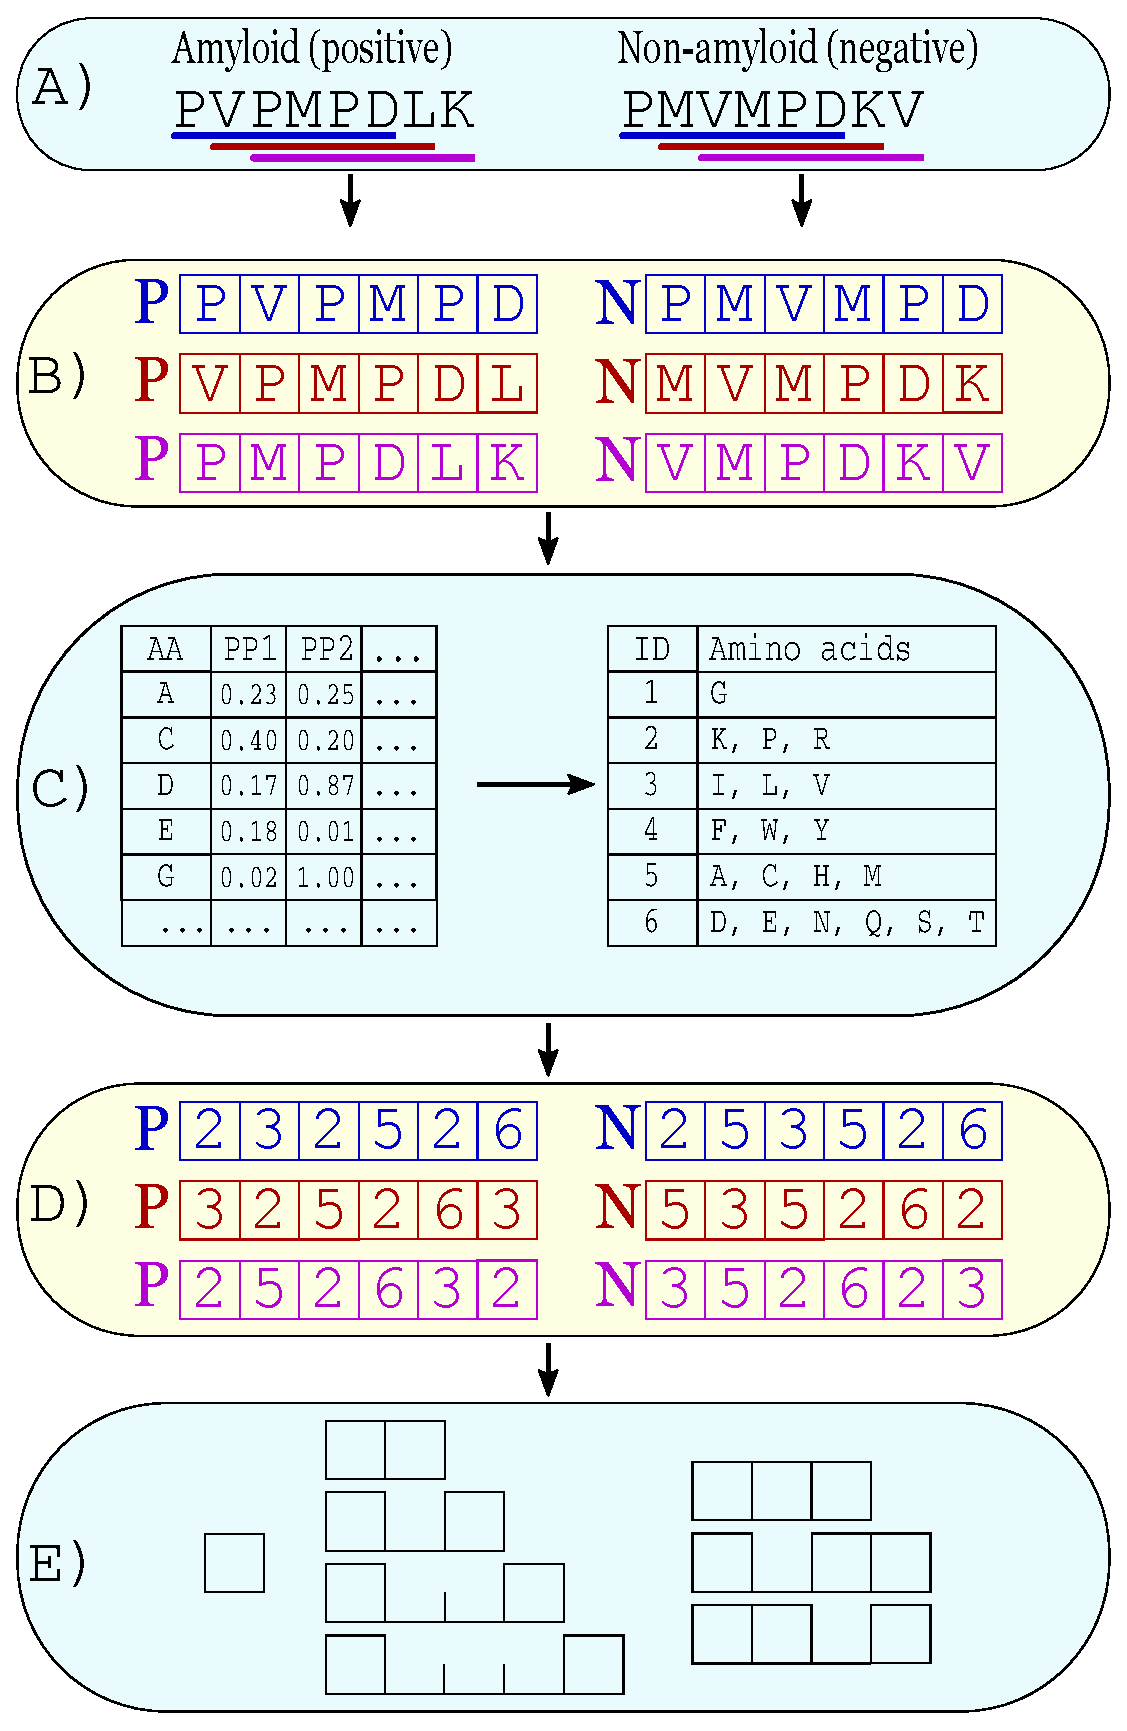
\includegraphics[width=\columnwidth]{figures/ngram_scheme.eps}} 
\caption{The scheme of n-gram extraction from studied peptide sequences. 
A) Source data: peptides with known amyloidogenicity status and indicated overlapping hexamers.
B) Extraction of the overlapping hexamers and ascription to them of the amyloidogenicity status taken from their source peptide (P-positive, N - negative). 
C) Clusterization of amino acids into an encoding using a combination of various
physicochemical properties (PP). 
D) Reduction of the amino acid alphabet in hexamers. 
E) Extraction of n-grams. From each hexamer, we extracted continuous n-grams with the 
length n = 1, 2 or 3. In addition, we selected 
gapped 2-grams with a gap of the length from 1 to 3 residues and gapped 
3-grams with a single gap between the first and the second or the second and 
the third element of the n-gram.
F) Selection of informative n-grams with Quick Permutation Test (QuiPT).
G) Training of a random forest classifier using n-grams selected in the previous step.}\label{fig:ngram_scheme} 
\end{figure}

  In the initial phase, we extracted overlapping hexamers from each peptide 
sequence. Each hexamer was tagged with the same etiquette (amyloid/nonamyloid) 
as the source peptide. (Fig.~\ref{fig:ngram_scheme} A and B). 

  Assuming that only a short part of the sequence in longer amyloids is 
responsible for amyloidogenicity, our method might result in many false 
positives in the training data set and in consequence yield inaccurate 
predictions as it was evaluated elsewhere \citep{kotulska_amyloid_2013}. To 
diminish this problem and facilitate the extraction of hot spots, we restricted the 
maximum length of peptides in training data set to fifteen amino acids.

  To further study the problem of the amyloidogenicity signal length, we 
created three learning sets with the sequences of different lengths 
(Tab.~\ref{tab:data_sets}). The smallest data set contained only the 
sequences of length 6. Assuming that the minimum length of the amyloidogenicity 
signal is the six residues, we can expect no false positive hexamers. Moreover, we 
created two training sets with the progressively more liberal limit of the 
maximum sequence length (6-10 residues and 6-15 residues).

\begin{table}
\centering
\small
\caption{Characteristics of training and test data sets used in the analysis.}
\label{tab:data_sets}
\begin{tabular}{cccll}
\toprule
Set & Sequence length & Status & Sequences & Hexamers \\ 
\midrule
\multirow{6}{*}{Training} & \multirow{2}{*}{6} & Non-amyloid & 841 & 841 
\\
 &  & \cellcolor[gray]{0.85}Amyloid & \cellcolor[gray]{0.85}247 & 
\cellcolor[gray]{0.85}247 \\
 \cline{2-5}
 & \multirow{2}{*}{{[}6,10{]}} & Non-amyloid & 964 & 1412 \\
 &  & \cellcolor[gray]{0.85}Amyloid & \cellcolor[gray]{0.85}312 & 
\cellcolor[gray]{0.85}475 \\
 \cline{2-5}
 & \multirow{2}{*}{{[}6,15{]}} & Non-amyloid & 992 & 1653 \\
 &  & \cellcolor[gray]{0.85}Amyloid & \cellcolor[gray]{0.85}342 & 
\cellcolor[gray]{0.85}720 \\
 \hline
 \hline
\multirow{8}{*}{Test} & \multirow{2}{*}{6} & Non-amyloid & 841 & 841 \\
 &  & \cellcolor[gray]{0.85}Amyloid & \cellcolor[gray]{0.85}247 & 
\cellcolor[gray]{0.85}247 \\
 \cline{2-5}
 & \multirow{2}{*}{{[}6,10{]}} & Non-amyloid & 123 & 571 \\
 &  & \cellcolor[gray]{0.85}Amyloid & \cellcolor[gray]{0.85}65 & 
\cellcolor[gray]{0.85}228 \\
 \cline{2-5}
 & \multirow{2}{*}{{[}11,15{]}} & Non-amyloid & 28 & 241 \\
 &  & \cellcolor[gray]{0.85}Amyloid & \cellcolor[gray]{0.85}30 & 
\cellcolor[gray]{0.85}245 \\
 \cline{2-5}
 & \multirow{2}{*}{{[}16,25{]}} & Non-amyloid & 41 & 571 \\
 &  & \cellcolor[gray]{0.85}Amyloid & \cellcolor[gray]{0.85}55 & 
\cellcolor[gray]{0.85}778 \\
 \bottomrule
\end{tabular}
\end{table}

  From each hexamer we extracted n-grams with the length of 1, 2 and 3. 
In the case of 2- and 3-grams, we separately analyzed continuous and gapped
n-grams. For 2-grams, we considered n-grams with the gap of the length from 1 to 3, 
whereas the 3-grams could contain a single gap between the first and the second or 
the second and the third position (see Fig.~\ref{fig:ngram_scheme}). The total number 
of n-grams depends on the the length of the encoding and is equal to 120, 260, 480 and 
798 for encodings of length 3, 4, 5 and 6 respectively.

  Furthermore, we repeated the procedure described above on two standard encodings 
derived from the literature to check if the process of amyloidogenicity does 
require nonstandard groupings of amino acids. We also added the full (unreduced) amino 
acid alphabet with 25,620 n-grams to assess the advantages of the amino acid encoding.

% * <pamac@smorfland.uni.wroc.pl> 2016-05-26T17:32:31.343Z:
%
% Iloma n-gramami bywały opisywane heksamery. To nie jest jasno opisane. Takze pozniej jak jest klasyfikowanie heksamerow, to ne ma nic o n-gramach, a przeciez na nich opieraly sie analizy. Trzeba napisac, ze nimi byly opisywane heksamery.
%
% ^ <michalburdukiewicz@gmail.com> 2016-06-06T08:26:52.851Z:
%
% opis jest w paragrafie: "From each hexamer we extracted..."
%
% ^.

\subsection{Quick Permutation Test (QuiPT)}

  All n-grams extracted from the hexamers in the training data set were 
filtered using the Quick Permutation Test with the information gain 
(mutual information) as the criterion of the importance of a specific n-gram. 
Only n-grams with the p-value smaller than 0.05 were assumed to be informative.

The permutation tests are commonly used for filtering important n-grams. 
However, they are computationally expensive and as a result, they often become 
one of the most limiting factors for these kinds of analyses. 
The Quick Permutation Test effectively filters n-gram features without performing 
a huge number of permutations. Let us consider a contingency table for a target 
$y$ and a feature $x$. For example, the entry $n_{1,0}$ is the number of cases 
when the target is $1$ and the feature is $0$.

\begin{center}
\begin{tabular}{ | c || c | c | c | }
  \hline			
  target / feature & 1 & 0 & total\\ \hline
 1 & $n_{1,1}$ & $n_{1,0}$ & $n_{1,\bigcdot}$ \\
 0 & $n_{0,1}$ & $n_{0,0}$ & $n_{0,\bigcdot}$ \\ \hline
 total & $n_{\bigcdot,1}$ & $n_{\bigcdot,0}$ & $n$ \\
  \hline  
\end{tabular} 
\end{center}

  Under the hypothesis that $x$ an $y$ are independent, the probability of 
observing such a contingency table is given by the multinomial distribution. 
The idea of permutation test is to reshuffle labels of features and targets  but 
keeping the fixed total number of positives for features and targets . When we 
impose this constraint on the multinomial distribution, then the probability of occurrence 
for a given contingency table depends only on one entry, i.e., $n_{1,1}$, which is 
fairly easy to compute. After computing Information Gain (IG) for each possible 
value of $n_{1,1} \in [0,\min(n_{\bigcdot, 1}; n_{1, \bigcdot})]$, we get the 
distribution of Information Gain under hypothesis that the target and feature are 
independent. We reject null hypothesis, when IG for the tested feature is above 
the required quantile from the IG distribution.

  The analytic formula for the distribution enables to perform the
permutation test much quicker. Furthermore, we get exact quantiles even for 
extreme tails of the distribution, which is not guaranteed by the random 
permutations. For example, for the test with $\alpha=10^{-8}$, which 
can often occur in the corrections for multiple testing, the standard deviation of quantile 
estimate in permutation test, $\frac{p(1-p)}{m}$, is roughly equal to $\alpha$ itself even for 
a huge number of permutations like $m=10^8$.

  In the context of n-gram data, we can further speed up our algorithm. Note 
that test statistics depends only on $n_{\cdot, 1}$, i.e., the number of positive cases in the 
feature when the target $y$ is common for testing all n-gram features . Although we test millions 
of features, there are only a few distributions that we need to compute because the usually number 
of positives in n-gram feature is small. We take advantage of this fact and we compute quantiles 
only for the handful of distributions. Therefore complexity of our algorithm is roughly equal $O(n\cdot p)$.

  Lastly, let us point out that QuiPT is very similar to Fisher's exact test. 
From the derivation provided in, e.g.~\citep{lehmann_testing_2008}, it becomes 
obvious that QuiPT is a heuristics for an unsolved problem of a two-tailed 
Fisher's exact test. In this heuristics, the extremity of a contingency table is 
defined by its Information Gain.

\subsection{Random forest classifier}

During the learning stage, random forest classifier was trained on the n-grams drawn 
from overlapping hexamers considering only n-grams selected by QuiPT. We grown forest with 
default parameters: 500 trees and the number of variables to possibly split at in each 
node equal to the (rounded down) square root of the total number of variables. The employed 
random forest implementation is using ranger \textbf{R} package~\citep{wright_ranger:_2015}.

  The predictor separately considered all hexamers coming from a single peptide. If at least 
one hexamer extracted from a peptide was assessed as amyloidogenic, the whole sequence was 
denoted as amyloid. Otherwise, the peptide was classified as non-amyloid. The results were 
next compared with the known etiquette of the peptides to compute the performance measures.


\subsection{Cross-validation and selection of the best-performing encoding}

The ability to correctly predict amyloidogenicity of peptides was assessed during 
the five-fold cross-validation. The peptides were assigned randomly to subsamples. 
Since this approach may result in the uneven number of hexamers in the subsamples 
(longer peptides yields more hexamers than shorter ones), we repeated the 
cross-validation fifteen times for each classifier to obtain more precise estimates 
of performance measures. 

  To evaluate if our classifiers are able to use decision rules extracted from 
sequences of given length to correctly classify longer or shorter sequences, we 
cross-validation.
% * <pamac@smorfland.uni.wroc.pl> 2016-05-26T17:34:31.688Z:
%
% To cos niedokonczone zdanie.
%
% ^ <pamac@smorfland.uni.wroc.pl> 2016-05-26T17:35:44.199Z.
  
  To choose the most adequate amino acid encoding, we ranked the values of Area under 
Curve (AUC) for the particular classifiers (with rank 1 for the best AUC, rank 2 for the second best AUC and so on) and various ranges of sequence length in the testing data set. The encoding with the lowest sum of ranks from all sequence length categories was selected as the best one. For this encoding, we choose the range of peptides length in the training set that provided the best AUC in the cross-validation.
% * <pamac@smorfland.uni.wroc.pl> 2016-05-26T18:45:37.232Z:
%
% To niejasne. Jaki udzial w wyborze tego najlepszego mialy training sets. One tez maja rozna dlugosc sekwencji. Czy ten najlepszy tez byl srednio najlepszy dla tych roznych zbiorow treningowych? To ostanir zdanie nie jest jasane. Na jakiej zasadzie zostaly wybrane zkresy dlugoaci w zbiorze traningowym? Z niego wynik, ze byly tak dobierane, aby ten najlepszy byl najlepszy. Te zakresy sa opisane duzow wczesniej i z tamtego opisu to nie wynika.
%
% ^.

\subsection{Encoding distance}
To compare obtained encodings, we introduced the encoding distance, which is a measure defining the similarity between two encodings . It has zero value for identical encodings and grows with the differences between the encodings. This parameter enabled us to select the reduced alphabets that were very similar to the best one and verify if they also show the good prediction performance.

  We define the encoding distance as the minimum number of amino acids that 
have to be moved between subgroups of the encoding \textit{a} to make it identical 
to the encoding \textit{b} (the order of subgroups in encodings and the order of amino acids in groups 
are not important). This measure was further scaled by a factor reflecting how 
much moving amino acids between groups altered the mean value of physicochemical properties in the group. 

To compute the scale factor $s$ for the encoding distance between 
the encoding \textit{a} with $n$ subgroups (enumerated with $i$) and the encoding \textit{b} with $m$ 
subgroups (enumerated with $j$), we first calculated $p_i$ and $q_j$, i.e. the mean values of physicochemical 
properties of all amino acids for each subgroup. 
% * <pamac@smorfland.uni.wroc.pl> 2016-05-26T18:03:57.604Z:
%
% To niejasne. Czy i oraz j to podgrupy dla jednego encoding czy podgrupy z dwoch roznych porownywanych encodings czyly a i b?
%
% ^ <pamac@smorfland.uni.wroc.pl> 2016-05-26T18:05:18.175Z.
The factor $s$ between encodings $a$ and $b$ is equal to: 

$$
s_{ab} = \sum^n_{i = 1}  \left( \min_{j=1,\dots,m} \; \; \sum^L_{l=1} \sqrt{ (p_{i,l} - q_{j,l})^2} \right)
$$

where $L$ is the number of considered physicochemical properties. Hence, 
the normalizing factor may be interpreted as the minimum change of the mean physicochemical properties between groups.

\subsection{Benchmark of AmyloGram}

The best-performing encoding chosen during the cross-validation was later used 
to train AmyloGram, n-gram based predictor of peptide amyloidogenicity.

  To compare the performance of AmyloGram and other predictors of amyloids 
we used external data set \textit{pep424}~\citep{walsh_pasta_2014}. Since some 
peptides were common for both \textit{pep424} and AmyLoad, we removed them from 
the training data set. After the purification, the learning data set for purposes of 
benchmark consisted of 269 positive sequences and 746 negative sequences longer 
than five and shorter than fifteen residues.

  We removed peptides shorter than five amino acids from the \textit{pep424} data set 
as they are shorter that minimum length assumed in the our model of amyloidogenicity.
This change should not have affect the comparison as only five sequences were eliminated 
(around 1\% of the original data set). Besides the classifier based on the reduced amino acid alphabet, 
we also benchmarked three predictors based on the full 20-amino acid alphabet 
learned on n-grams extracted from sequences with different length ranges to separately 
assess the benefit of using only the n-gram analysis without the reduction of amino 
acid alphabet.


% * <pamac@smorfland.uni.wroc.pl> 2016-05-26T18:23:59.560Z:
%
% To cos niejasne. Na poczatku jest opisany final set z innymi liczbami. Ile jest w zbiorze uczacym, a ile w testowym.
%
% ^ <pamac@smorfland.uni.wroc.pl> 2016-05-26T18:25:03.061Z.
% * <pamac@smorfland.uni.wroc.pl> 2016-05-26T19:13:35.990Z:
%
% Generalnie, te metody troche niejasni opisane.
%
% ^ <pamac@smorfland.uni.wroc.pl> 2016-05-26T19:14:10.200Z.
\section{Results and discussion}

\subsection{Performance of the best encoding}
% * <pamac@smorfland.uni.wroc.pl> 2016-05-26T19:22:13.000Z:
%
% Wszedzie zamiast testing chyba powinno byc tested. Tez na rysunkach.
%
% ^ <michalburdukiewicz@gmail.com> 2016-06-06T08:26:10.670Z:
%
% poprawiono na "test"
%
% ^.
\begin{figure*}[!tpb]
\centerline{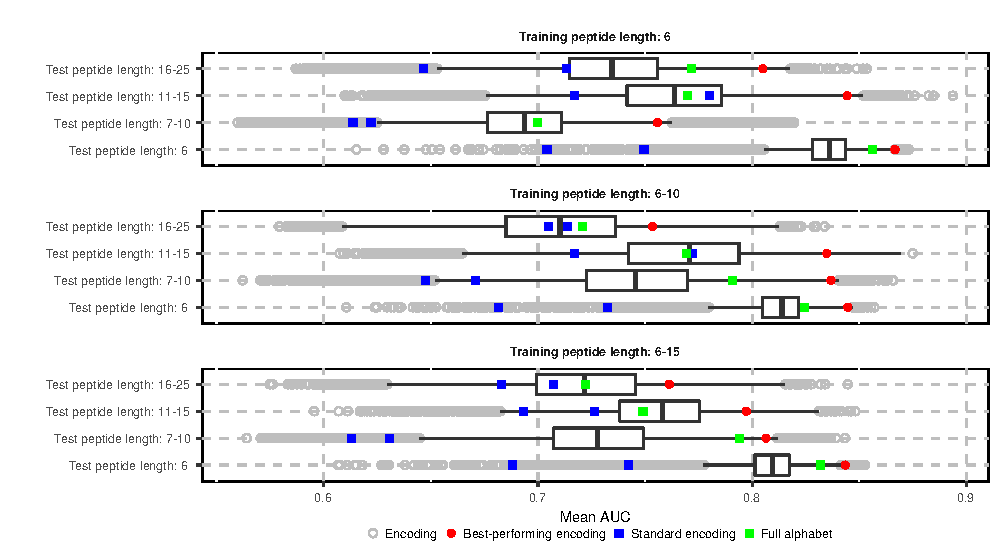
\includegraphics{figures/AUC_boxplot.eps}}
\caption{Distribution of mean AUC values of classifiers with various encodings for every possible combination of training and testing data set including different lengths of sequences. 
The left and right hinges of boxes correspond to the 0.25 and 0.75 quartiles. 
The bar inside the box represents the median. The gray circles correspond to the
encodings with the AUC outside the 0.95 confidence interval. The best-performing encoding was best by average for various ranges of sequence length in the testing data set.
% Red circle: classifier employing best encoding of amino acid. Green square: 
% classifier using full amino acid alphabet. Blue square: classifiers employing 
% encodings from literature.
}\label{fig:AUC_boxplot} 
\end{figure*}
% * <pamac@smorfland.uni.wroc.pl> 2016-05-26T18:54:12.528Z:
%
% Tego encoding from literature bym nie wyroznial, jesli to nie jest jakis osobny klasyfikator. Inne AAindeksy tez sa z jakies literatury.
%
% ^ <pamac@smorfland.uni.wroc.pl> 2016-05-26T18:54:49.283Z.
\begin{figure*}[!tpb]
\centerline{\includegraphics{figures/sesp_plot.png}}
\caption{Sensitivity and specificity of classifiers with various encodings for 
every possible combination of sequence lengths in the training and testing data sets.
%Red 
%circle: classifier employing best encoding of amino acid. Green square: 
%classifier using full amino acid alphabet. Blue square: classifiers employing 
%encodings from literature. 
The classifier based on the best-performing encoding always have 
good specificity and sensitivity.}\label{fig:sesp_plot}
\end{figure*}

% * <pamac@smorfland.uni.wroc.pl> 2016-05-26T18:56:04.414Z:
%
% Tego encoding from literature bym nie wyroznial, jesli to nie jest jakis osobny klasyfikator. Inne AAindeksy tez sa z jakies literatury
%
% ^ <pamac@smorfland.uni.wroc.pl> 2016-05-26T18:56:11.423Z.

The selected encoding performed better than other reduced alphabets considering 
all ranges of sequence lengths in the training and testing data set. It had the AUC
always in the fourth quartile of other encodings (Fig.~\ref{fig:AUC_boxplot}).   The best encoding reached the highest values of AUC (=...) in the recognition of the shortest sequences (with 6 residues) when the training set also consisted of the sequences with the same length. It may result most probably from the homogenity of the short peptides . Nevertheless, the results were quite comparable even if the training set contained longer sequences. By average, the majority of encodings behaved like the selected encoding and also received higher AUC for the shorter tested sequences than for the longer ones.
For the best-performing encoding, the most problematic was the correct prediction of the 
amyloidogenicity in the longest peptide from 16 to 25 residues, when the algorithm was learned also on longer peptides (6-10 and 6-15 data sets).

 The weakest performance measured by AUC for sequences longer than 15 amino acids results from difficulties in extraction of  the important discriminating features related with more complex organization of longer amylogenic peptides. In such peptides, only a very specific region of residues 
might be responsible for the creation of harmful aggregates. In this case, when 
overlapping hexamers are extracted, only part of them may carry the true signal 
of amyloidogenicity but all of them are marked as amyloids. However, despite this problem, the 
overall prediction of classifiers learned on the long sequences was still 
adequate, with the median values of AUC higher than 0.7 for every testing set. 

  In addition to the high AUC, the best encoding had also very good sensitivity 
and specificity regardless of the length of sequences in training and tested 
set (Fig.~\ref{fig:sesp_plot}). The classifiers trained on the peptides with the 
length 6 tended to have the best specificity, whereas predictors learned on the 
long sequences had the best sensitivity. Although the classifiers trained on the
six-residue-long sequences had generally the better AUC, their training on the sequences 
from six to ten residues seems to yield the most balanced classifiers 
with the optimal sensitivity and specificity.

  We also evaluated classifiers based on the full (i.e., unreduced) amino acid alphabet. In most 
cases, they were also placed in the fourth quartile of AUC value 
(Fig.~\ref{fig:AUC_boxplot}). Nevertheless, they never predicted 
amyloidogenicity better than the best classifier based on the reduced alphabet. It indicates that despite 
a lot of information present in the full alphabet, the encoding allows better 
generalization of the prediction rules and in the consequence a better 
performance.

  Similarly to the best-performing encoding, the sensitivity of classifiers 
based on the full amino acid alphabet decreased with the length of sequences in 
the training data set (Fig.~\ref{fig:sesp_plot}). Furthermore, these 
classifiers always seemed to  have one of the worst sensitivities among all analyzed 
predictors, especially when tested on the longer amyloids. It means that using the 
full amino acid alphabet it was easier to point the non-amyloidogenic sequences 
instead of amyloids.

  The standard encodings found in the literature perform significantly worse than other 
analyzed encodings in all categories. It indicates that the descriptive divisions 
of amino acids do not create groups suitable for the recognition of amyloids. This 
observation is well-supported by the specificity-sensitivity plot 
(Fig.~\ref{fig:sesp_plot}), where classifiers trained with this encodings of 
amino acids groups belong to the worst performers.
% * <pamac@smorfland.uni.wroc.pl> 2016-05-26T22:07:49.243Z:
%
% Nie jest dla mnie jasne co to sa te kodowania z litratury.
%
% ^ <pamac@smorfland.uni.wroc.pl> 2016-05-26T22:08:20.197Z.

\subsection{The best-performing encoding and important n-grams}

\begin{figure}[!tpb]
\centerline{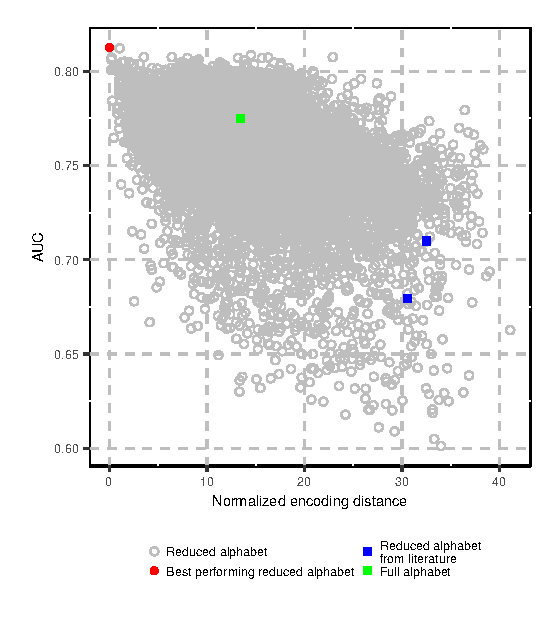
\includegraphics{figures/ed_AUC.eps}}
\caption{The encoding distance and AUC of the reduced alphabets studied in the 
cross-validation. 
%Red circle: classifier employing best encoding of amino acid. Green square: 
%classifier using full amino acid alphabet. Blue square: classifiers employing 
%encodings from literature. 
Classifiers with the smallest encoding distance to the best classifier have 
the highest AUC.}\label{fig:ed_AUC}
\end{figure}

% latex table generated in R 3.2.3 by xtable 1.8-2 package
% Tue Mar  8 14:20:53 2016
\begin{table}[ht]
\centering
\caption{The best-performing encoding.} 
\label{tab:best_enc}
\begin{tabular}{cl}
\toprule
Subgroup ID & Amino acids \\ 
\midrule
  1 & G \\ 
\rowcolor[gray]{0.85}  2 & K, P, R \\ 
3 & I, L, V \\ 
\rowcolor[gray]{0.85}  4 & F, W, Y \\ 
5 & A, C, H, M \\ 
\rowcolor[gray]{0.85}  6 & D, E, N, Q, S, T \\ 
\bottomrule
\end{tabular}
\end{table}


\begin{figure}[!tpb]
\centerline{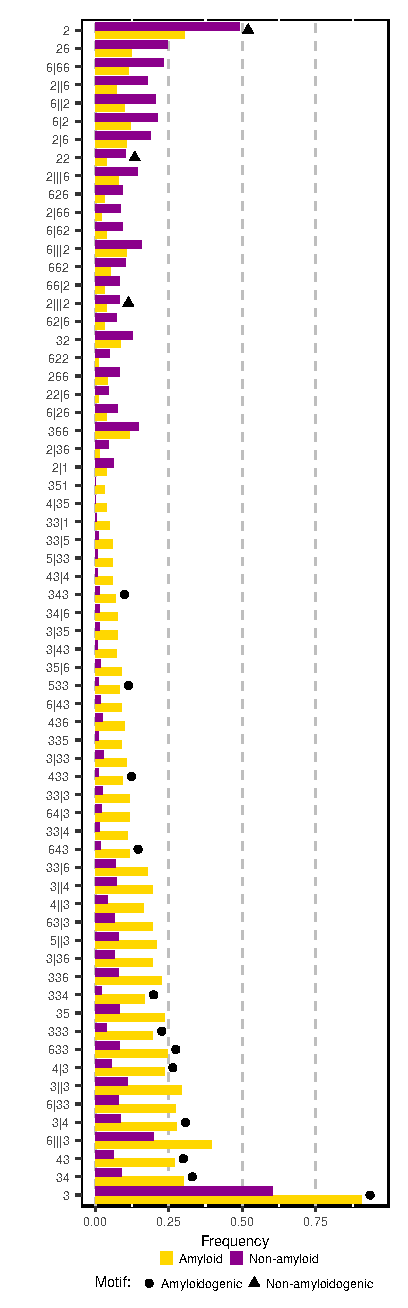
\includegraphics{figures/ngrams.eps}}
\caption{The frequency of important n-grams used by the best-performing 
classifier 
in amyloid and non-amyloid sequences. The elements of n-grams 
are amino acids encoded using the best-performing reduced amino acid 
alphabet (see Tab.~\ref{tab:best_enc}). A vertical bar 
represents a gap in a n-gram between its elements. The frequency was computed using the total number of occurrences divided by the number of possible n-grams of this length.
Dots and triangles denote n-grams occurring in motifs found in respectively amyloidogenic and non-amyloidogenic sequences~\citep{paz_sequence_2004}.}\label{fig:ngrams}
\end{figure}
% * <pamac@smorfland.uni.wroc.pl> 2016-05-26T23:01:59.166Z:
% Z czego ta czestosc? Kiedy sumuje sie do 100%? Moze to posortowac wg roznic w czestosciach miedzy dwoma grupami, albo wg czestosci amyloidow.
%
% ^.
% * <michalburdukiewicz@gmail.com> 2016-06-06T08:21:58.121Z:
%
% czestosc przeliczono na poszczegolne n-gramy i posortowano
%
% ^.

  In total, eleven combinations of physicochemical properties created the best 
performing encoding. Only four features appeared in all combinations: hydrophobicity index~\citep{argos_structural_1982}, average flexibility indices~\citep{bhaskaran_positional_1988}, polarizability 
parameter~\citep{charton_structural_1982} and thermodynamic $\beta$-sheet propensity~\citep{kim_thermodynamic_1993}.

The best encoding chosen in the analysis consists of six amino acid subgroups, which are characterized by distinct and specific properties (Tab.~\ref{tab:best_enc}). The 3rd subgroup contains strongly hydrophobic amino acids. In the 4th subgroup, the amino acids show also aromatic properties. On the other hand, the most hydrophilic amino acids are in the 2nd and 6th soubgroups . The former includes two clear basic amino acids, whereas the latter two acidic and four polar residues. The first subgroup includes only glycine, which is the smallest amino acid and the most flexible.  By average, quite flexible amino acids are also present in the 2nd subgroup, whereas the least flexible amino acids are in the subgroup 4 and 5. The glycine has also the lowest propensity to form $\beta$-sheet and the subgroups 3 and 4 largest.

To compare  the best-performing encoding to other encodings, we calculated encoding distances between  them (Fig.~\ref{fig:ed_AUC}). To compute the scale 
factor, we used normalized values of described above four features. The value of AUC is significantly lower for more distant encodings ($-0.437$ Pearson's correlation coefficient, p-value smaller than $2.2 \times 10^{-16}$). Such relationship indicates that the best-performing encoding was not found by chance and inclusion of properties reflected by this encoding improves the prediction of amyloids.

  We selected 65 n-grams that obtained p-values smaller than 0.05 in QuiPT test in all repetitions of cross-validation regardless of the length of sequences in the training set (see Fig.~\ref{fig:ngrams}). The frequency of the n-grams was computed for all sequences derived from AmyLoad database. The n-grams typical of amyloidogenic sequences (with the highest frequency in amyloids) incorporate 
mostly highly hydrophobic amino acids with tendency to form $\beta$-structures , from 
subgroups 3 and 4. The n-grams occurring frequently in amyloids have often 
 repeats of amino acids from the subgroup 3, suggesting that the presence of these amino acids in vicinity might be one of the most effective predictors of amyloidogenicity.

On the other hand, n-grams typical of non-amyloidogenic peptides have mostly amino acids 
belonging to subgroups 2 and 6 which include strongly hydrophilic and highly flexible amino acids, which may hamper forming $\beta$-structures.

\subsection{Benchmark of AmyloGram}

% latex table generated in R 3.2.3 by xtable 1.8-2 package
% Tue Mar  8 14:17:55 2016
\begin{table}[ht]
\centering
\small
\caption{Results of benchmark on \textit{pep424} data set for PASTA2, 
FoldAmyloid, AmyloGram and random forest predictor learned on n-grams extracted 
for full amino acid alphabet from the sequences with the length specified in 
the brackets (FA).} 
\label{tab:bench_summary}
\begin{tabular}{ccccc}
  \toprule
Classifier & AUC & MCC & Sensitivity & Specificity \\ 
  \midrule
AmyloGram & \textbf{0.8972} & \textbf{0.6307} & 0.8658 & 0.7889 \\ 
   \rowcolor[gray]{0.85}full alphabet (6) & 0.8411 & 0.5427 & 0.4966 & 
\textbf{0.9593} \\ 
  full alphabet (6-10) & 0.8581 & 0.5698 & 0.7517 & 0.8259 \\ 
   \rowcolor[gray]{0.85}full alphabet (6-15) & 0.8610 & 0.5490 & 0.8188 & 
0.7519 \\ 
\hline \hline
  PASTA2 & 0.8550 & 0.4291 & 0.3826 & 0.9519 \\ 
   \rowcolor[gray]{0.85}FoldAmyloid & 0.7351 & 0.4526 & 0.7517 & 0.7185 \\ 
  APPNN & 0.8343 & 0.5823 & \textbf{0.8859} & 0.7222 \\ 
   \bottomrule
\end{tabular}
\end{table}

The benchmark covered AmyloGram as well as three peer-reviewed predictors of 
amyloidogenicity: PASTA2~\citep{walsh_pasta_2014}, 
FoldAmyloid~\citep{garbuzynskiy_foldamyloid:_2010} and 
APPNN~\citep{familia_prediction_2015}. Other classifiers published before were 
not included in the benchmark because their performance on \textit{pep424} 
data set is already known and lower than the performance of PASTA2 and 
FoldAmyloid~\citep{walsh_pasta_2014}.

  We analyzed Area Under the Curve (AUC), Matthew's Correlation Coefficient 
(MCC), sensitivity and specificity (see Tab.~\ref{tab:bench_summary}). We used 
default settings for FoldAmyloid and PASTA2 evaluated input data in the 
'Peptides' mode.

  Since PASTA2 does not return a probability of belonging to specific category, 
we normalized the output data to compute the AUC values. The advised 
energy threshold (-5) was also normalized in the same manner and used as 
cut-off in computations of specificity, sensitivity and MCC. The resulting 
value of specificity 0.9519 is close to the value provided by authors (0.95) and assures 
correctness of our computations. For other classifiers, we assumed 0.5 
cut-off.
    
  In the case of the studied data set, the n-gram extraction method appeared efficient enough to 
produce classifiers able to outperformed the published methods. AmyloGram showed the highest AUC and MCC among all tested classifiers. It had lower specificity than two n-gram classifiers trained on the full alphabet but still outperformed two other published method in this category. It is important to 
highlight that AmyloGram is the most balanced among all analyzed classifiers, 
having the best specificity/sensitivity trade-off, as indicated by the value of MCC.
 
  The specificity of AmyloGram is lower than the specificity of PASTA2 but it
is a consequence of the usage of the threshold value optimized for 0.95 
specificity for the latter. If we assume for the AmyloGram the same threshold for the specificity, our classifier will
have still higher sensitivity (0.5518) than PASTA2. Therefore, if we assume thresholds to both predictors detect true non-amyloids with the same accurateness, AmyloGram predicts more true amyloids. 

  Two of three classifiers based on n-gram and  trained on the full alphabet had also AUC higher than PASTA2 and all three were more successful than FoldAmyloid as well as APPNN. They also maintained  the high specificity as seen previously during cross-validation. However, they generally performed worse than the classifier based on reduced amino acid alphabet.

  Among all considered predictors of amyloidogenicity, APPNN had the highest 
sensitivity. Nevertheless, its AUC was worse than AUCs of all n-gram-based 
predictors as well as PASTA2 indicating lower overall performance.

  AmyloGram is trained to predict amyloidogenic, not amyloidic regions. Hence, we did not tested it on \textit{reg33} data set, which is commonly used to detect the performance in prediction of all regions participating in the amyloid aggregation~\citep{tsolis_consensus_2013}.
   
\subsection{AmyloGram web server}

Our software is accessible as the web server under address \url{www.smorfland.uni.wroc.pl/amylogram/}. AmyloGram is also
accessible in the batch mode as the R package (ADDRESS). 

\section{Conclusion}

Thanks to the reduction of amino acid alphabet, we were able to create the 
efficient predictor of amyloidogenic sequences called AmyloGram. One of the 
strength of our approach is its highly interpretable outcome, which hopefully 
sheds new light on the process of amyloid aggregation.

  The idea of using the encodings is a proven concept. We employed it in our 
innovative framework to generate and validate several thousands of possible 
amino acid encodings. Due to this approach, we were able to specify important 
physicochemical properties that define the best-performing alphabet and thereby extract features associated with amyloidogenicity, such as hydrophobicity and tendency to forming $\beta$-sheets.  In addition to them, we discovered a new property,  i.e. flexibility.  

  Our analysis was completed with the extraction of important n-grams, which 
might be interpreted as short motifs highly relevant to amyloidogenicity or 
non-amyloidogenicity of peptides. Sixty five important n-grams revealed that mostly 
alifatic and nonpolar amino acids (isoleucine, leucine and valine) together with aromatic and also hydrophobic amino acids (phenylalanine, tyrosine, tryptophan) are good predictors of amyloids.

  Since the best-performing classifier was trained on the alphabet consisting of  
six amino acid groups, it still outperformed predictors learning on the raw amino acid sequences and is enough to find n-grams separating efficiently amyloids and non-amyloids. 


\section*{Funding}

Computations were carried out in Wroclaw Center for Networking 
and Supercomputing (\url{http://www.wcss.pl}) and funded by the
institutional grant No. 347.

This research was funded by the KNOW Consortium and
National Science Center (2015/17/N/NZ2/01845).

\bibliographystyle{NAR-natbib}
\bibliography{amyloids}
\end{document}
